%%=============================================================================
%% Methodologie
%%=============================================================================

\chapter{Methodologie}
\label{ch:methodologie}

%% TODO: Hoe ben je te werk gegaan? Verdeel je onderzoek in grote fasen, en
%% licht in elke fase toe welke stappen je gevolgd hebt. Verantwoord waarom je
%% op deze manier te werk gegaan bent. Je moet kunnen aantonen dat je de best
%% mogelijke manier toegepast hebt om een antwoord te vinden op de
%% onderzoeksvraag.
Dit hoofdstuk beschrijft hoe men het best te werk kan gaan voor de daadwerkelijke opzet van een eenvoudig, kleinschalig blockchain gebaseerd stemsysteem. De implementatie die hier wordt besproken gebeurt op basis van de verschillende technieken die werden toegelicht in het vorig hoofdstuk. Er wordt gekozen voor het Ethereum blockchain platform als ontwikkelomgeving, deze keuze gebeurt op basis van sectie \ref{sec:ethereum-en-smart-contracts} van het vorige hoofdstuk. In dit hoofdstuk bieden we verder antwoord op de onderzoeksvragen \textit{wat de praktikaliteit van een blockchain gebaseerd stemsysteem is}, \textit{hoe haalbaar een blockchain gebaseerd stemsysteem is} en tenslotte ook \textit{of er sprake van een onoverkomelijk schaalbaarheidsprobleem}.

\section{Benodigdheden}
\label{sec:benodigdheden}
De volgende zaken dienen geïnstalleerd te worden voor men van start kan gaan met het implementeren van Ethereum blockchain applicatie:
\begin{itemize}
	\item{Node.js}
	\item{npm}
	\item{Truffle}
	\item{Ganache}
	\item{Metamask}
\end{itemize}
Daarnaast heeft men ook nodig:
\begin{itemize}
	\item{Een IDE naar keuze met syntax ondersteuning voor Solidity}
	\item{Google Chrome}
\end{itemize}

\subsection{ node en npm}
Node.js is een veelgebruikte Runtime-omgeving waarmee Javascript op ieder platform uitgevoerd kan worden, zonder dat daar een browser voor nodig is. Npm is een pakketbeheerder voor Javascript code. Npm zit standaard in Node.js en is `s werelds grootste softwareregister. Open source-ontwikkelaars wereldwijd gebruiken het om pakketten te delen, veel organisaties gebruiken npm om ook hun privéontwikkeling te beheren (\ref{fig:nodejs}).\footnote{Verkregen en vertaald van https://docs.npmjs.com/about-npm/}

Eenmaal node\footnote{node met npm is verkrijgbaar via https://nodejs.org} en npm\footnote{npm is ook apart verkrijgbaar via https://www.npmjs.com/get-npm} geïnstalleerd zijn, verifieert men de installatie via het console-commando: \textit{node -v} . Bij correcte installatie geeft dit de huidige node versie terug, bijvoorbeeld \textit{v10.15.1}. 

\begin{figure}
	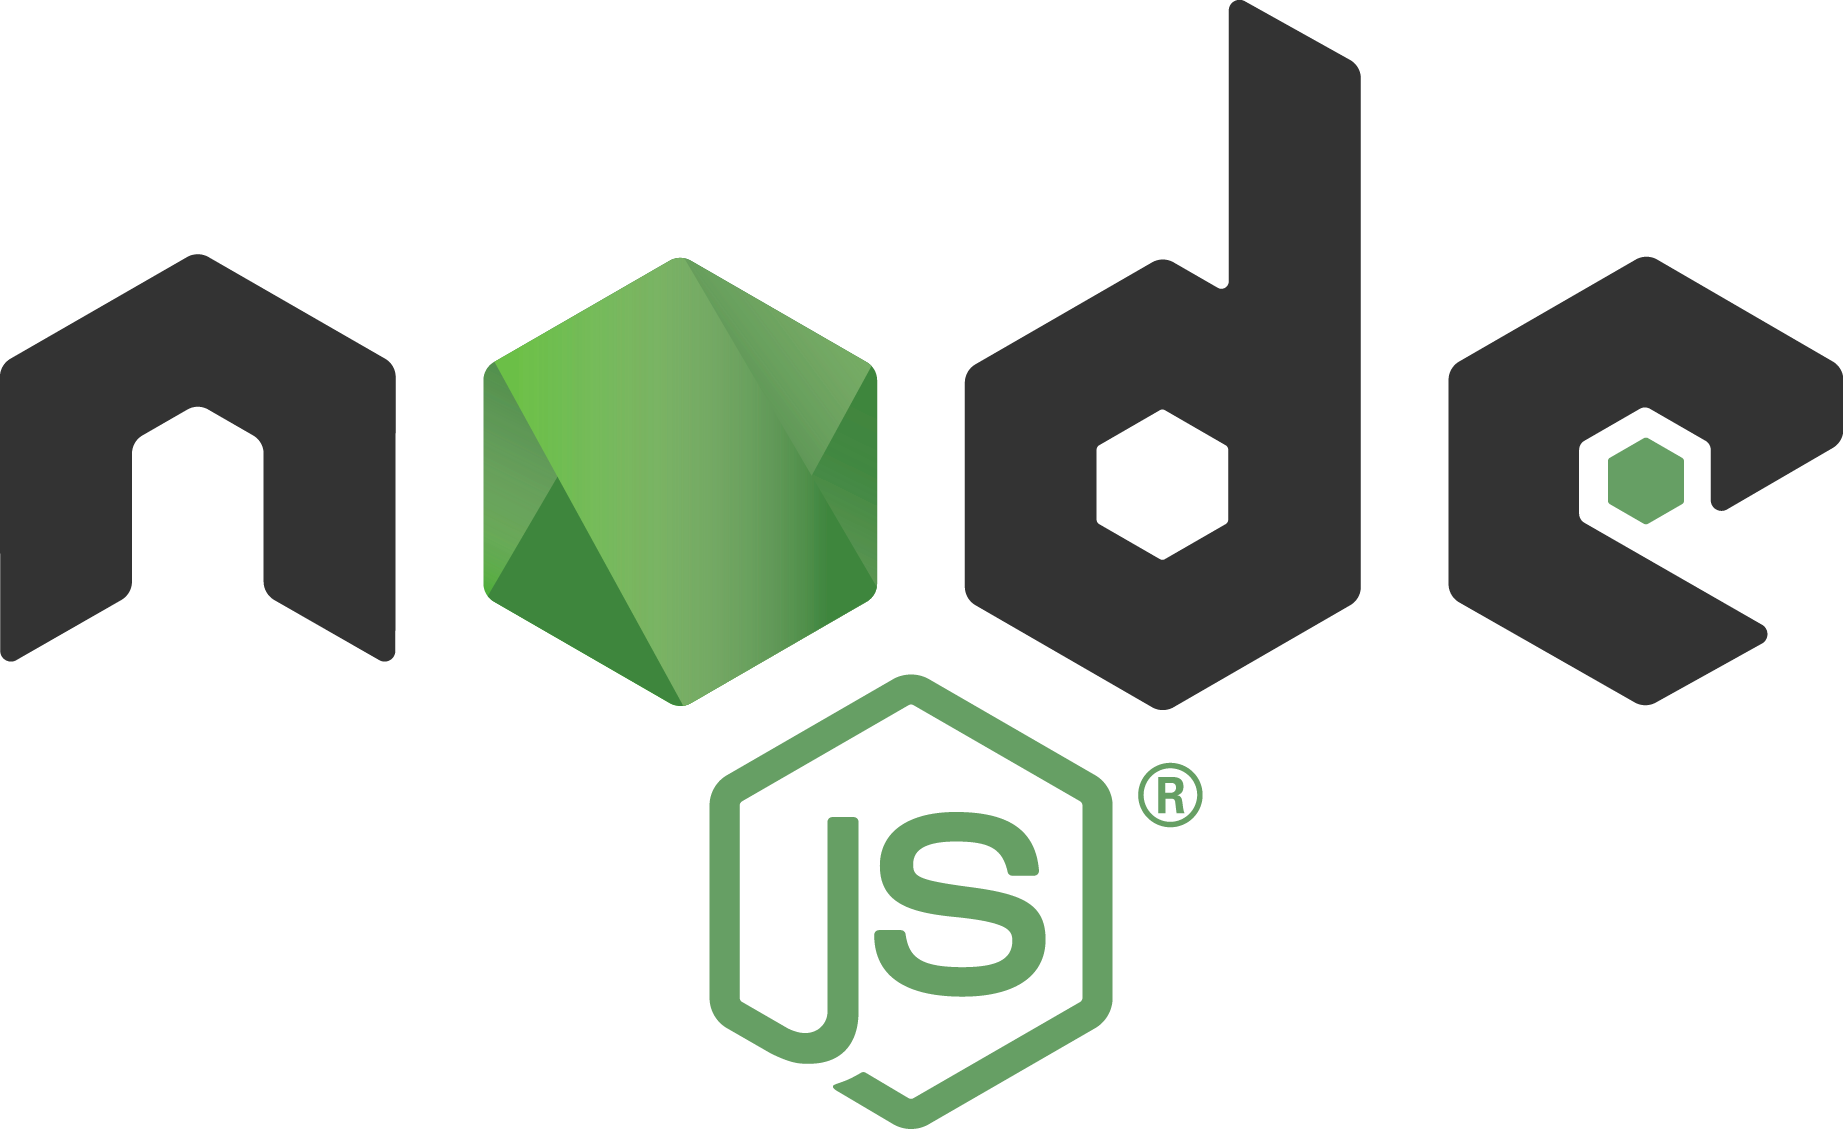
\includegraphics[width=\linewidth/2]{img/nodejs.png}
	
\includegraphics[width=\linewidth/2]{img/npm.png}
	\caption{De Node.js en npm logo's}
	\label{fig:nodejs}
\end{figure}

\subsection{Truffle}
Truffle is een ontwikkelomgeving, testframework en asset pipline, gericht op het versoepelen van het Ethereum ontwikkelproces. Het bevat ook verschillende code-templates die als basis kunnen worden gebruikt om gedecentraliseerde applicaties te ontwikkelen.

Truffle kan eenvoudig geïnstalleerd worden via npm (mits dit al geïnstalleerd is) met het console-commando: \textit{npm install truffle}.

\subsection{Ganache}
Ganache\footnote{Ganache is verkrijgbaar via https://www.trufflesuite.com/ganache} is een applicatie die ontwikkelaars in staat stelt om een private Ethereum-blockchain op te zetten. Deze blockchain wordt gebruikt gedurende de volledige ontwikkelperiode. Op deze manier kan men kosteloos smart-contracts ontwikkelen en testen. Indien men direct op de hoofdketen zou ontwikkelen zou er aan iedere actie een transactie kost verbonden zijn. Ganache biedt ons 10 externe accounts met adressen op onze lokale Ethereum-blockchain. Elke account is vooraf geladen met 100 nep-ether.

\subsection{Metamask}
Metamask\footnote{Metamask is verkrijgbaar via https://metamask.io of via https://chrome.google.com/webstore} is een plugin voor Google Chrome die ontwikkelaars toelaat Ethereum dApps uit te voeren in de browser zonder zelf een node te moeten zijn in het netwerk, zonder dus de volledige blockchain te moeten downloaden.

\begin{figure}
	
\includegraphics[width=\linewidth]{img/metamask-truffle-ganache.png}
	\caption{Truffle, Metamask en Ganache logo's}
	\label{fig:metamask-truffle-ganache}
\end{figure}









